\subsubsection{Tables}

Pour créer des tables de résultats, j'ai lancé des campagnes de test avec des instances de trois tailles différentes : 500 noeuds, 1000 noeuds et la ville entière de Tours (44000 noeuds). Ces trois instances sont détaillées table \ref{tab:instances}.

\begin{table}[!h]
\centering
\caption{Détail des instances utilisées. Pour le nombre de POI, le filtre est celui détaillé section \ref{sect:poi}.}
\vspace{0.2cm}
\begin{tabular}{|c|c|c|c|c|}
\hline
Instance & Card(noeuds) & Card(arcs) & Card(POI) & Card(carreaux) \\  
\hline
$\texttt{500N\_0}$ & 498 & 1222 & 22 & 90 \\
\hline 
$\texttt{1000N\_0}$ & 1000 & 2517 & 41 & 235 \\
\hline 
$\texttt{Tours}$ & 43668 & 108431 & 3684 & 8831 \\
\hline 
\end{tabular}
\label{tab:instances}
\end{table}

Ces instances sont des quartiers de Tours, qui m'ont été gentillement fournies par Félix Repusseau, un doctorant du LIFAT travaillant sur des problématiques similaires.

L'objectif d'avoir plusieurs instances était de voir le comportement des algorithmes dans différents contextes, pour mieux couvrir les anomalies éventuelles, et d'avoir des résultats pour différentes tailles de graphe. Les modèles exacts sont très lents sur la métropole entière de Tours, pour pouvoir les comparer aux heuristiques sur des valeurs de paramètres (la distance maximale, le budget et le niveau LTS maximal) un peu réalistes, il fallait des instances plus petites.

J'ai fait des tests avec des paramètres non réalistes, juste pour avoir des résultats de comparaison de l'efficacité des modèles. J'ai aussi fait des tests avec des paramètres plus réalistes, pour voir ce qu'il se passait dans un cas proche d'une application réelle.

Les instances étant trop couteuses pour être lancées en local (Processeur Intel(R) Pentium(R) CPU 5405U @ 2.30GHz, 8 Go de mémoire RAM), mes tests ont été effectués sur le Mésocentre de Calcul CaSciModOT \cite{cas}. C'est un centre régional de calcul parallèle de taille intermédiaire entre des stations de travail et les grands centres nationaux (CINES, IDRIS, CCRT). Il permet de fournir à l'ensemble des partenaires de la fédération CaScIModOT une grappe possédant une puissance de calcul hautes performances. Les calculs sont lancés sur un processeur AMD Epyc 7702 à 2GHz.

\paragraph{Ecart de valeur objective entre la visibilité exacte et la visibilité PCC}

\begin{table}[!ht]
\centering
\caption{Valeur objective (\emph{Objective Value}, OV) du modèle exact sur la visbilité des PCC, la fonction objective étant la minimisation de PPOI (critère \ref{criterepoi} dans \ref{criteresopti}), pour l'instance \texttt{500N\_0}}
\vspace{0.5cm}
\begin{tabular}{|l|l|l|p{2cm}|p{2cm}|p{2cm}|p{2cm}|}
\hline
B & dmax & LTS & OV initiale sur la
visibilité exacte & OV initiale sur la
visibilité PCC & OV finale sur la visibilité exacte & OV finale sur la visibilité PCC \\
\hline
1000 & 400 & 1 & 2 & 2 & 27 & 27 \\
1000 & 500 & 1 & 2 & 2 & 30 & 28 \\
1000 & 400 & 1.375 & 81 & 68 & 101 & 99 \\
1000 & 500 & 1.375 & 132 & 110 & 173 & 170 \\
1000 & 400 & 1.3 & 21 & 15 & 63 & 58 \\
1000 & 500 & 1.3 & 29 & 20 & 87 & 75 \\
2000 & 1000 & 1 & 2 & 2 & 73 & 73 \\
2000 & 2000 & 1 & 2 & 2 & 83 & 83 \\
2000 & 400 & 1 & 2 & 2 & 43 & 43 \\
2000 & 800 & 1 & 2 & 2 & 65 & 65 \\
2000 & 800 & 1.375 & 319 & 215 & 449 & 429 \\
2000 & 1000 & 1.3 & 75 & 36 & 316 & 265 \\
2000 & 2000 & 1.3 & 154 & 41 & 721 & 378 \\
2000 & 400 & 1.3 & 21 & 15 & 80 & 76 \\
2000 & 800 & 1.3 & 57 & 30 & 236 & 199 \\
\hline
\end{tabular}
\label{tab:nbppoi}
\end{table}

Voir table \ref{tab:nbppoi}
\textcolor{red}{commenter etc}

\paragraph{Comparaison de l'efficacité des différents modèles}

Nous pouvons comparer l'efficacité des modèles grâce aux tables 

Pour les tables , l'efficacité est calculée par erreur relative \cite{erreur_relative}. Plus exactement, elle est donnée par :



\begin{table}[H]
\centering
\caption{Résultats pour l'optimisation sur le nombre de ppoi (critère \ref{criterepoi} dans \ref{criteresopti}), instance comprenant 500 noeuds (\texttt{500N\_0})}
\label{tab:res500}
\vspace{0.5cm}
\begin{tabular}{|c|c|c|c|p{2cm}|p{2cm}|p{2cm}|p{2cm}|p{2cm}|}
\hline
id & B & dmax & LTS & temps pris par
le modèle exact sur la visibilité exacte (1) & temps pris par le modèle exact sur la visibilité PCC (2) & temps pris par
l'heuristique \ref{hpcc} avec tri sur (3) & erreur relative de
(2) par rapport à (1) & erreur relative de
(3) par rapport à (2) \\
\hline
1 & 1000 & 1000 & 1 &  & 3.0729 & 0.0054 &  & 2.356 \\
2 & 1000 & 400 & 1 & 71.1325 & 0.2221 & 0.0004 & 2.564 & 8.75 \\
3 & 1000 & 1000 & 1.3 &  & 2.0355 & 0.007 &  & 8.378 \\
4 & 1000 & 400 & 1.3 & 14.7487 & 0.1978 & 0.0005 & 25.714 & 16.327 \\
5 & 1000 & 1000 & 1.375 &  & 1.4007 & 0.0085 &  & 12.426 \\
6 & 1000 & 400 & 1.375 & 2.7308 & 0.1304 & 0.0006 & 200.0 & 25.0 \\
7 & 2000 & 1000 & 1 &  & 4.4433 & 0.0054 &  & 5.919 \\
8 & 2000 & 400 & 1 & 197.2866 & 0.2319 & 0.0005 & 4.918 & 14.062 \\
9 & 2000 & 1000 & 1.3 &  & 1.8768 & 0.0073 &  & 24.667 \\
10 & 2000 & 400 & 1.3 & 74.8399 & 0.1359 & 0.0005 & 50.0 & 25.806 \\
11 & 2000 & 1000 & 1.375 &  & 1.3584 & 0.0091 &  & 18.75 \\
12 & 2000 & 400 & 1.375 & 1.4945 & 0.0598 & 0.0006 &  &  \\
\hline
\end{tabular}
\end{table}

J'ai crée des tables plus détaillées, comparant plus de paramètres \textcolor{red}{mettre en annexe ?}

% Tester les modèles sur différentes tailles d'instances m'a permis de constater que l'efficacité des modèles ne varie pas avec la taille de l'instance, mais seulement avec la taille des paramètres (??).


Des valeurs réalistes de $\texttt{dmax}$ sont de 5km (2 miles, la valeur utilisée dans \cite{kent_karner}), ou après échange avec Lou-Ann Deniau, $1,4$km, la distance moyenne qu'un cycliste effectue pour se rendre à un POI.

La plus grande distance $\texttt{dmax}$ que j'ai testée pour l'instance de Tours, avec le modèle exact sur la visibilité exacte, est de 400m. Au delà de cela, le calcul nécéssitait plus de 512go de mémoire. C'est éloigné des valeurs de $\texttt{dmax}$ sur lesquelles on souhaiterait que le modèle fonctionne.

Pour l'instance de Tours, le modèle exact sur la visibilité PCC fonctionne sur $\texttt{dmax}=1,4$km, mais pas sur $\texttt{dmax}=5$km.



\subsubsection{Cartes}

\subsection{Difficultés rencontrées}

\paragraph{Déboguage}

Une des difficultés majeures de ce stage a été le déboguage des modèles et des fonctions. Pour avoir des résultats intéressants, il faut un graphe d'au moins 100 noeuds. Il est donc nécessaire d'avoir des instances de test, pour vérifier que les fonctions ont bien le comportement attendu.

Un problème se pose, il est difficile d'être exhaustif sur tous les cas particuliers pouvant créer des erreurs lorsqu'on crée une instance de test.

Ainsi, j'avais des erreurs qui apparaissaient seulement dans des grands graphes, pour lesquels faire tourner l'algorithme à la main est fastidieux et difficile. J'ai néanmoins dû me rabattre sur cette méthode pour déboguer certaines erreurs, mes instances tests me servaient seulement à vérifier le comportement de mes fonctions lors du développement. Lorsque je repérais un bug sur une instance précise, je lançais le débugger C++ jusqu'à trouver l'erreur.

Déboguer les modèles CPLEX est aussi difficile, de manière générale. Le fichier .lp généré, permettant de voir les variables et contraintes crées par CPLEX, fait déjà plusieurs centaines de lignes pour un graphe d'une dizaine de noeuds.

\paragraph{Gérer les campagnes de test}

J'effectuais mes campagnes de test sur CaSciModOT, 

Voir 2 visibilités différentes

\paragraph{Danger d'un arc aménagé}

Mis à 0 pour des raisons de simplification, pourrait potentiellement poser des problèmes par la suite.

Vu que je suis pas un expert en XML et que mon stage était davantage axé sur la partie optimisation que sur la partie amélioration de l'application  

\paragraph{Arrondir danger conflit cohérence réelle cartographes et optimisation}

Les données qui m'étaient fournies pour calculer le niveau LTS sur un tronçon étaient deux nombres, la distance en mètres du tronçon et un nombre "danger", dont le ratio $\fFrac{\text{danger}}{\text{distance}}$ était censé appartenir à l'ensemble $R=\{1; 1.15; 1.3; 1.375; 1.45; 1.75\}$. Ces données étaient stockées dans le fichier .csv des arcs du réseau.

Il arrivait que ce ratio soit légèrement supérieur à l'une de ces valeurs, par exemple $1.3+10^{-8}$. Lors des applications réelles de ce programme, on veut optimiser en fournissant un ratio maximum appartenant à $R$. Cela pose alors problème, parce qu'un arc ayant un ratio très légèrement supérieur à une valeur de $R$ sera traité comme étant à aménager, alors qu'il s'agit juste d'un problème d'arrondi et qu'on le considère déjà comme empruntable.

J'ai donc ajouté une tolérance lors de l'optimisation, pour que les arcs légèrement supérieurs à une valeur $v$ de l'ensemble $R$ soient traités comme s'ils étaient à $v$. 

Sur les tables que j'ai fournies, \textcolor{blue}{la tolérance était à \texttt{10e-4}.} \textcolor{red}{pas encore, elle est à 0}

\paragraph{Travailler sur deux projets}

J'ai repris deux projets déjà entamés par le LIFAT, Bike Accessibility (optimisation d'un réseau cyclable) et Chemins Equitables (visualisation d'indicateurs d'équités). J'ai ensuite dù faire communiquer ces deux projets. 

Dans les projets Bike Accessibility et Chemins Equitables, des étapes se succédaient entre ces deux projets, voir parfois certaines étapes étaient effectuées sur les 2 projets à la fois (par exemple, le calcul des PM est implicitement fait sur le projet Bike Accessibility, puisque on calcule déjà la possibilité d'emprunter chaque chemin). Il fallait alors s'assurer de la cohérence des résultats trouvés sur chacun de ces projets. 

Mon objectif a été de faire mes modifications au maximum sur le projet Bike Accessibility, pour réduire le risque d'erreur entre la communication entre les projets. C'est cette logique qui m'a poussé, pour l'optimisation sur la diversité de catégories de POI, j'ai choisi de filtrer les POI dans le parser de Bike Accessibility, plutôt que de générer un nouveau fichier POI dans l'application Chemins Equitables et d'utiliser celui là (l'autre avantage étant de pouvoir faire l'optimisation sur le même jeu de données directement). Mon objectif était ensuite de générer sur Bike Accessibility un nouveau fichier POI contenant seulement les POI sur lesquels l'optimisation a été faite (ceux d'une des catégories conservées).

L'idéal aurait été de tout générer dans le projet Bike Accessibility, pour réduire le risque d'erreur à cause d'incohérences (par exemple, les arrondis du facteur LTS, décrit au paragraphe précédent, n'étaient pas les mêmes sur les deux projets).

Or, insérer toute la partie génération de données post-optimisation, ainsi que la partie génération de PM avant et après optimisation, dans le projet Bike Accessibility, de manière propre et facilement expandable si l'on rajoute des modèles, était une tâche compliquée. Le développement de toutes ces étapes sur l'application Chemins Equitables a été faite en 2 mois par deux stagiaires à la fois

Ma solution a été de vérifier à la main la cohérence des deux projets, et d'ajouter des fonctions de test à certains endroits. Par exemple, sur la figure \ref{fig:nb_poi_compa}, on peut voir une comparaison visuelle des résultats de ces deux projets, pour le nombre de POI accessibles par chaque carreaux.

\begin{figure}[H]
\centering
    \begin{tabular}{cc}    
        \begin{minipage}[t]{2.5in}
        \centering
        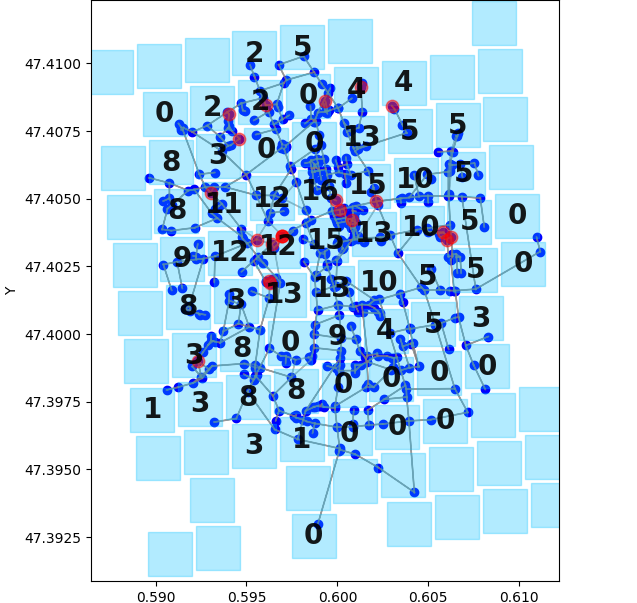
\includegraphics[height=2in]{nb_poi_BA.png}
        % \label{fig:task1_l1}
        \end{minipage}
    %%    
        \begin{minipage}[t]{2.5in}
        \centering
        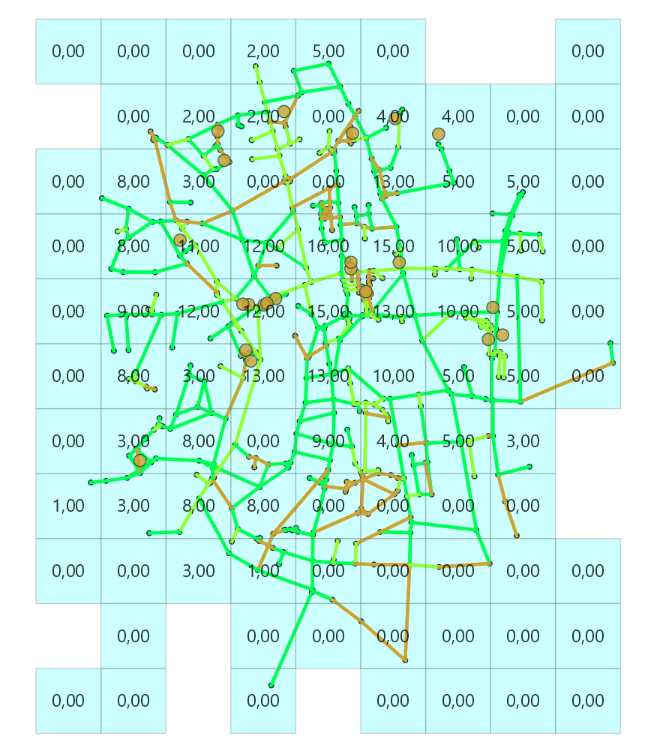
\includegraphics[height=2in]{nb_poi_CE.png}
        % \label{fig:task1_cpu}
        \end{minipage}
    \end{tabular}
    \caption{Un des tests pour vérifier la cohérence des deux projets. A gauche, le nombre de POI accessibles par carreau INSEE pour le projet Bike Accessibility. A droite, le nombre de POI accessibles par carreau INSEE pour le projet Chemins Equitables. Pour la ville de Fondettes, dans l'agglomération de Tours.}
    \label{fig:nb_poi_compa}
\end{figure}

J'ai codé dans le projet Bike Accessibility la génération d'un PM (pour l'heuristique sur la diversité de catégories), et j'ai comparé les résultats donnés avec le même PM codé sur l'application Chemins Equitables. En revanche, on ne peut pas être certain d'être exhaustif en vérifiant complètement seulement certains éléments.

Quant aux POI, j'ai fini par coder un filtre pour afficher seulement les POI pertinents sur les cartes, pour avoir des cartes exploitables par les cartographes (mais utiliser ce fichier POI nécéssitait de renommer des choses à la main, alors que ces étapes sont automatisées sinon. En somme, ce n'est pas une solution durable).
